%% =============================================================================
%% VERA: Vascular Explainable Retinopathy Assessment  --  IEEE conference paper
%% Build:  python generate_ieee_paper_figures.py   (creates figures/)
%%         pdflatex vera_ieee_conference.tex  (run twice)
%% =============================================================================
\documentclass[conference]{IEEEtran}

\usepackage{cite}
\usepackage{amsmath,amssymb,amsfonts}
\usepackage{graphicx}
\usepackage{textcomp}
\usepackage{xcolor}
\usepackage{booktabs}
\usepackage{array}
\usepackage{tikz}
\usepackage{microtype}

% ---- shorthand --------------------------------------------------------------
\newcommand{\vera}{VERA}
\newcommand{\gcpp}{Grad-CAM++}
\newcommand{\sov}{S_{\mathrm{overlap}}}
\newcommand{\rvasc}{R_{\mathrm{vasc}}}
\newcommand{\qwk}{\mathcal{L}_{\mathrm{QWK}}}
\newcommand{\Ihat}{\hat{I}}

\begin{document}

\title{VERA: Vascular Explainable Retinopathy Assessment via Multi-Modal 4-Channel Fusion and Grounded Saliency for Clinical Decision Support}

\author{
\IEEEauthorblockN{Yeasir Ramim}
\IEEEauthorblockA{\textit{Dept. of CSE}\\
\textit{United International University}\\
Dhaka, Bangladesh\\
yramim223103@bscse.uiu.ac.bd}
\and
\IEEEauthorblockN{Shopnil Saha}
\IEEEauthorblockA{\textit{Dept. of CSE}\\
\textit{United International University}\\
Dhaka, Bangladesh\\
ssaha223529@bscse.uiu.ac.bd}
\and
\IEEEauthorblockN{Meheruna Afsar Jenin}
\IEEEauthorblockA{\textit{Dept. of CSE}\\
\textit{United International University}\\
Dhaka, Bangladesh\\
mjenin223789@bscse.uiu.ac.bd}
}

\maketitle

% =============================================================================
\begin{abstract}
Diabetic retinopathy (DR) is a leading cause of preventable blindness in working-age adults. Convolutional networks trained on 3-channel RGB fundus photographs reach high benchmark scores but are prone to shortcut learning, relying on optical artifacts such as border vignetting, illumination gradients, and pigmentation instead of microvascular lesions, and their qualitative saliency maps are rarely verified. We present VERA (Vascular Explainable Retinopathy Assessment), an explainable-by-design clinical decision support system for 5-class ICDR severity grading. VERA (i)~fuses an illumination-normalized fundus image with a continuous vessel-probability map, obtained from multi-scale Frangi vesselness and morphological top-hat filtering, into a 4-channel input $[R,G,B,V]$; (ii)~adapts the ResNet-50 stem so that vascular structure is encoded from the first layer; (iii)~trains with a differentiable surrogate quadratic weighted kappa (QWK) loss that penalizes distant grade errors; and (iv)~quantifies where the network looks with a Continuous Vessel-Attention Overlap Score computed on Grad-CAM++ maps. On APTOS 2019, EyePACS, and Messidor-2, VERA reaches 88.2\% accuracy and $\kappa=0.893$ ($+0.089$ over the RGB baseline), 95.8\% sensitivity and 94.2\% specificity for referable DR (AUC 0.982), and no errors larger than one grade. The overlap score rises from 0.221 to 0.342 ($+54.7\%$), indicating that attention is anchored on the vasculature rather than on background artifacts. The pipeline is packaged as a clinician-in-the-loop studio with ETDRS 4-2-1 rule evaluation, macular-threat triage, and PDF report generation at 42~ms per scan.
\end{abstract}

\begin{IEEEkeywords}
Diabetic retinopathy, medical artificial intelligence, shortcut learning, multi-modal feature fusion, Grad-CAM++, vessel segmentation, clinical decision support systems, quadratic weighted kappa.
\end{IEEEkeywords}

% =============================================================================
\section{Introduction}

Diabetic retinopathy (DR) is a chronic, progressive microvascular complication of diabetes mellitus and the leading cause of preventable blindness among working-age adults worldwide \cite{cheung2010,yau2012}; an estimated 103 million people were affected in 2020 \cite{teo2021}. Chronic hyperglycemia causes retinal capillary basement-membrane thickening, pericyte loss, and focal capillary dilations termed \textbf{microaneurysms (MAs)}. As capillary non-perfusion progresses, localized ischemia triggers intraretinal hemorrhages, lipid leakage (hard exudates), cotton wool spots (nerve-fiber-layer infarcts), and ultimately abnormal \textbf{neovascularization}, which can culminate in vitreous hemorrhage or tractional retinal detachment \cite{fong2004}.

Severity is graded on the International Clinical Diabetic Retinopathy (ICDR) five-stage scale \cite{wilkinson2003}:
\begin{itemize}
\item \textbf{Grade 0 (No DR):} no retinal microvascular lesions;
\item \textbf{Grade 1 (Mild NPDR):} microaneurysms only;
\item \textbf{Grade 2 (Moderate NPDR):} more than microaneurysms alone (blot hemorrhages and/or hard exudates) but less than severe NPDR;
\item \textbf{Grade 3 (Severe NPDR):} the Early Treatment Diabetic Retinopathy Study (ETDRS) \textbf{4-2-1 rule}: hemorrhages in 4 quadrants, venous beading in $\ge 2$ quadrants, or prominent IRMA in $\ge 1$ quadrant;
\item \textbf{Grade 4 (Proliferative DR, PDR):} neovascularization (NVD/NVE) or preretinal/vitreous hemorrhage.
\end{itemize}
Early detection and timely treatment (panretinal photocoagulation or anti-VEGF therapy) reduce the incidence of severe visual loss by over 95\% \cite{etdrs10}. Population-scale screening is nevertheless bottlenecked by the global shortage of medical retina specialists, so treatable non-proliferative disease can advance silently to irreversible impairment.

\begin{figure*}[!t]
\centering
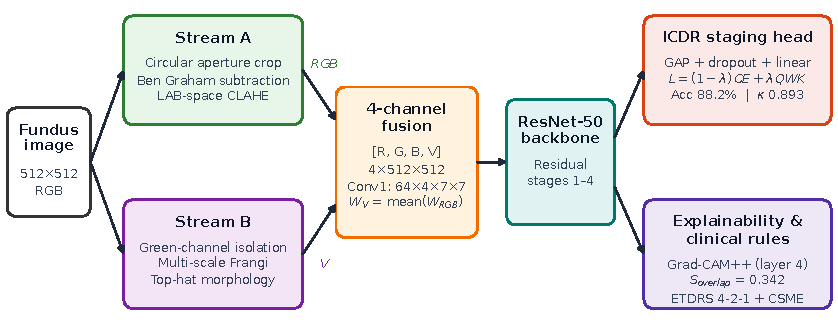
\includegraphics[width=\textwidth]{figures/fig1_system_architecture.pdf}
\caption{End-to-end architecture of VERA. Stream~A normalizes illumination (circular aperture crop, Ben Graham color subtraction, CLAHE); Stream~B extracts the retinal vascular tree (Frangi vesselness and morphological top-hat). The resulting 4-channel tensor $[R,G,B,V]$ enters a ResNet-50 with a modified stem, trained with a joint cross-entropy and surrogate QWK loss, and is paired with \gcpp{} grounding and automated ETDRS 4-2-1 / macular-threat evaluation.}
\label{fig:arch}
\end{figure*}

\subsection{Shortcut Learning in Retinal AI}
Many deep CNNs have been proposed to relieve this screening burden \cite{gulshan2016,ting2017,gargeya2017}. Networks trained on raw RGB fundus photographs, however, are exposed to \textbf{shortcut learning} \cite{geirhos2020}: they exploit statistical heuristics in the training distribution, such as aperture-border vignetting, illumination gradients, corneal flash reflections, or choroidal pigmentation, rather than retino-vascular lesions. Deployed on heterogeneous imaging hardware, such models can label healthy eyes as diseased from peripheral illumination artifacts alone, eroding clinician trust.

Post-hoc interpretability is also limited. Standard Grad-CAM \cite{selvaraju2017} yields coarse, qualitative saliency blobs; in multi-lesion disease it averages gradients globally and tends to attenuate secondary punctate lesions, so clinicians cannot verify quantitatively whether the network's attention aligns with genuine vascular pathology.

\subsection{Contributions}
This paper presents \textbf{VERA}, an anatomically grounded, explainable-by-design framework. Our contributions are:
\begin{enumerate}
\item \textbf{Explicit 4-channel early fusion $[R,G,B,V]$.} An auxiliary vascular stream extracts a continuous vessel map that is fused with the preprocessed RGB image. By redesigning the stem convolution of a ResNet-50, we impose an anatomical inductive bias at layer~1, encouraging the network to place lesions in the context of the vascular tree.
\item \textbf{Differentiable surrogate QWK loss.} A continuous relaxation of Quadratic Weighted Kappa lets us optimize clinical ordinal agreement directly and penalize distant grade errors heavily.
\item \textbf{Quantitative anti-shortcut explainability ($\sov$).} The Continuous Vessel-Attention Overlap Score is a bounded index in $[0,1]$ that measures the spatial alignment between \gcpp{} activations and the vascular map.
\item \textbf{Specialist rule automation and macular triage.} An ETDRS 4-2-1 quadrant engine and a foveal-avascular-zone (FAZ) proximity algorithm flag severe NPDR and clinically significant macular edema (CSME).
\item \textbf{Clinical translation.} The verified architecture is packaged as an interactive decision-support system that produces multi-panel 300-DPI A4 consultation reports with digital specialist sign-off, at 42~ms per scan.
\end{enumerate}

% =============================================================================
\section{Related Work}

\subsection{Deep Learning for DR Classification}
Gulshan et al.\ \cite{gulshan2016} demonstrated specialist-level sensitivity and specificity with deep CNNs on EyePACS and Messidor-2. Later work explored higher-capacity backbones, including ResNet \cite{he2016}, DenseNet \cite{huang2017}, and EfficientNet \cite{tan2019}, and ordinal formulations such as soft-label encoding and threshold regression \cite{gao2020}. Nearly all of these frameworks treat DR grading as an ungrounded 3-channel RGB vision task, leaving them vulnerable to background shortcuts and camera-specific domain shift.

\subsection{Retinal Vessel Segmentation and Structural Priors}
Vessel caliber, branching angle, tortuosity, and capillary drop-out reflect systemic microvascular compromise \cite{fraz2012}. Vessel extraction methods divide into unsupervised filtering, such as multi-scale Frangi filters \cite{frangi1998} and Gabor wavelets \cite{soares2006}, and supervised networks such as U-Net \cite{ronneberger2015} trained on DRIVE and CHASE\_DB1. Although vessel segmentation is well studied in isolation, its use as an explicit inductive prior for ordinal DR staging remains underexplored. Multi-task frameworks typically add vessel segmentation as an auxiliary loss, which does not guarantee that the primary classifier grounds its attention on the extracted vasculature.

\subsection{Saliency and Explainability Grounding}
Interpretability in medical imaging commonly relies on CAM \cite{zhou2016} and Grad-CAM \cite{selvaraju2017}. Grad-CAM averages positive gradients uniformly over spatial positions, which dilutes the response when several micro-lesions co-occur. Chattopadhay et al.\ proposed Grad-CAM++ \cite{chattopadhay2018}, which uses higher-order derivatives to weight each pixel and so handles multiple lesion instances. Even so, saliency maps remain largely qualitative in ophthalmic literature. VERA closes this gap with a formal metric that quantifies attention alignment against verified anatomical vasculature.

% =============================================================================
\section{Proposed Methodology}

The VERA pipeline (Fig.~\ref{fig:arch}) runs two synchronized streams: Stream~A (color and illumination normalization) and Stream~B (microvascular extraction). Their outputs are fused into one tensor for classification, grounding, and rule verification.

\subsection{Stream A: Input Validation and Preprocessing}
Raw fundus photographs vary widely in color temperature, aperture size, and illumination falloff. Stream~A applies four sequential operations.
\begin{enumerate}
\item \textbf{Input validation.} The image $I\in\mathbb{R}^{H\times W\times 3}$ is checked for plausible retinal color. Because hemoglobin absorbs strongly in the blue-green range, foreground pixels must satisfy $(\mu_R{+}1)/(\mu_B{+}1)>1.2$, $(\mu_R{+}1)/(\mu_G{+}1)>0.95$, and a warm-hue (HSV) proportion above $0.45$. The variance of the Laplacian of the green channel must also exceed 5.0 ($\mathrm{Var}(\nabla^2 G)>5.0$) to confirm vascular edge contrast. Images failing these tests are rejected as ungradable.
\item \textbf{Circular aperture cropping.} Black borders are removed by thresholding gray intensity ($I_{\mathrm{gray}}>10$), locating the circular field of view, and cropping with a 2-px margin.
\item \textbf{Ben Graham local color normalization.} To neutralize camera-specific illumination we apply local color subtraction \cite{graham2015}:
\begin{equation}
\begin{split}
\Ihat=\mathrm{Clip}\big(&4I-4\,\mathrm{GaussianBlur}(I,\sigma{=}10)\\
&+128,\,0,\,255\big).
\end{split}
\label{eq:graham}
\end{equation}
Pixels outside the field of view are masked back to zero.
\item \textbf{Luminance-channel CLAHE.} To enhance low-contrast microaneurysms without chromatic distortion, the image is converted to CIE LAB and CLAHE (clip limit 2.0, $8{\times}8$ tiles) is applied to the $L^*$ channel only before conversion back to RGB.
\end{enumerate}

\subsection{Stream B: Microvascular Extraction}
Stream~B produces a continuous vessel-probability map $V\in[0,1]^{H\times W}$. Deep U-Nets could be used, but deterministic multi-scale filtering gives predictable behavior across heterogeneous clinical centers.
\begin{enumerate}
\item \textbf{Green-channel isolation.} The green channel $G$ gives the best contrast between hemoglobin-filled vessels and the background. Background variation is reduced by median illumination subtraction:
\begin{equation}
G_{\mathrm{norm}}=1.5\,G-0.5\,\mathrm{MedianBlur}(G,15).
\end{equation}
\item \textbf{Multi-scale top-hat transform.} With $I_{\mathrm{inv}}=255-G_{\mathrm{norm}}$ and an ensemble of elliptical structuring elements $K_s$, $s\in S=\{3,5,7,9\}$,
\begin{equation}
V_{\mathrm{tophat}}=\frac{1}{|S|}\sum_{s\in S}\big(I_{\mathrm{inv}}-I_{\mathrm{inv}}\circ K_s\big),
\end{equation}
where $\circ$ denotes morphological opening.
\item \textbf{Frangi vesselness.} Local tubular geometry is captured by the eigenvalues $|\lambda_1|\le|\lambda_2|$ of the Hessian $\mathcal{H}_\sigma=\nabla^2(G_{\mathrm{norm}}*\mathcal{G}_\sigma)$, with $\mathcal{G}_\sigma$ a Gaussian kernel:
\begin{align}
\mathcal{R}_B&=\frac{|\lambda_1|}{|\lambda_2|},\qquad \mathcal{S}=\sqrt{\lambda_1^2+\lambda_2^2},\\
\mathcal{V}_\sigma&=\begin{cases}
0, & \lambda_2>0,\\[2pt]
e^{-\mathcal{R}_B^2/2\beta^2}\big(1-e^{-\mathcal{S}^2/2c^2}\big), & \text{otherwise,}
\end{cases}
\end{align}
with $\beta=0.5$ and $c=15.0$. The response over $\sigma\in[1.0,3.0]$ is normalized to $[0,1]$ by power-law gamma scaling ($\gamma=0.85$).
\end{enumerate}

\subsection{4-Channel Early Feature Fusion}
Rather than concatenating features in late fully connected layers, VERA stacks the enhanced RGB image and the vessel map into one tensor,
\begin{equation}
\mathbf{X}_{\mathrm{fused}}=[R,G,B,V]\in\mathbb{R}^{4\times H\times W}.
\end{equation}
To feed it to an ImageNet-pretrained ResNet-50 while keeping the pretrained edge filters, the first convolution $\mathrm{Conv1}\in\mathbb{R}^{64\times3\times7\times7}$ is expanded to $64\times4\times7\times7$. The weights of the new fourth channel are initialized with the mean of the pretrained RGB filters,
\begin{equation}
\mathbf{W}_V=\tfrac{1}{3}\sum_{c\in\{R,G,B\}}\mathbf{W}_c .
\end{equation}
Channels 1--3 are normalized with ImageNet statistics ($\mu_{\mathrm{RGB}}=[0.485,0.456,0.406]$, $\sigma_{\mathrm{RGB}}=[0.229,0.224,0.225]$) and channel 4 with domain vascular statistics ($\mu_V=0.150$, $\sigma_V=0.250$).

\subsection{Differentiable Surrogate QWK Loss}
Standard cross-entropy penalizes confusing Grade~0 with Grade~1 exactly as much as confusing Grade~0 with Grade~4, although the latter risks missing proliferative disease and imminent blindness. The clinical reference metric is Quadratic Weighted Kappa,
\begin{equation}
\kappa=1-\frac{\sum_{i,j}W_{ij}O_{ij}}{\sum_{i,j}W_{ij}E_{ij}},\qquad W_{ij}=\frac{(i-j)^2}{(K-1)^2},
\end{equation}
where $K=5$, $O$ is the observed confusion matrix, and $E$ the expected matrix under marginal independence. Because $\arg\max$ predictions are non-differentiable, we use a continuous relaxation. Let $\mathbf{P}\in\mathbb{R}^{B\times K}$ be the softmax outputs for a mini-batch of size $B$ and $\mathbf{Y}$ the one-hot labels:
\begin{align}
\mathbf{O}_{\mathrm{soft}}&=\tfrac{1}{B}\mathbf{P}^{\top}\mathbf{Y},\qquad
\mathbf{E}_{\mathrm{soft}}=\mathbf{h}_p^{\top}\mathbf{h}_y,\\
\mathbf{h}_p&=\tfrac{1}{B}\textstyle\sum_{b}\mathbf{P}_b,\qquad
\mathbf{h}_y=\tfrac{1}{B}\textstyle\sum_{b}\mathbf{Y}_b,\\
\qwk&=\frac{\sum_{i,j}W_{ij}(\mathbf{O}_{\mathrm{soft}})_{ij}}{\sum_{i,j}W_{ij}(\mathbf{E}_{\mathrm{soft}})_{ij}+\epsilon}.
\end{align}
The total objective balances class calibration and ordinal distance,
\begin{equation}
\mathcal{L}_{\mathrm{total}}=(1-\lambda)\,\mathcal{L}_{\mathrm{CE}}+\lambda\,\qwk,
\label{eq:total}
\end{equation}
with $\lambda=0.40$ chosen empirically.

\subsection{Clinical Pathology Engines}
Beyond neural classification, VERA includes guideline-based rule engines.
\begin{enumerate}
\item \textbf{ETDRS 4-2-1 engine.} The fundus is divided into four quadrants relative to the optic disc and fovea: superior-temporal (ST), inferior-temporal (IT), superior-nasal (SN), and inferior-nasal (IN). Hemorrhages are segmented by morphological black-hat filtering of the green channel after vessel-tree subtraction. If $\ge20$ blot hemorrhages appear in all four quadrants, or venous beading is detected in $\ge2$ quadrants, VERA raises a \textbf{Severe NPDR (Grade~3)} alert, corresponding to a 50\% one-year risk of progression to proliferative disease \cite{wilkinson2003}.
\item \textbf{Macular threat triage (CSME/DME).} Diabetic macular edema causes central vision loss. VERA estimates the optic-disc (OD) diameter ($2R_{\mathrm{OD}}\approx1500\,\mu$m) and computes the Euclidean distance from each hard-exudate cluster $(x_{\mathrm{HE}},y_{\mathrm{HE}})$ to the FAZ center $(x_{\mathrm{FAZ}},y_{\mathrm{FAZ}})$:
\begin{equation}
d_{\mathrm{FAZ}}=\sqrt{(x_{\mathrm{HE}}-x_{\mathrm{FAZ}})^2+(y_{\mathrm{HE}}-y_{\mathrm{FAZ}})^2}.
\end{equation}
Exudates within one disc diameter ($d_{\mathrm{FAZ}}\le2R_{\mathrm{OD}}$) trigger a high-risk CSME warning; those between one and two disc diameters (DD) are flagged as moderate threat.
\item \textbf{Vascular morphometry.} Branching complexity is measured by the box-counting fractal dimension
\begin{equation}
D_{\mathrm{box}}=\lim_{\epsilon\to0}\frac{\log N(\epsilon)}{\log(1/\epsilon)}.
\end{equation}
Capillary drop-out lowers $D_{\mathrm{box}}$ below 1.38 (healthy range 1.40--1.48), whereas proliferative neovascular tufts raise it above 1.50.
\end{enumerate}

% =============================================================================
\section{Explainability and Quantitative Grounding}

\begin{figure*}[!t]
\centering
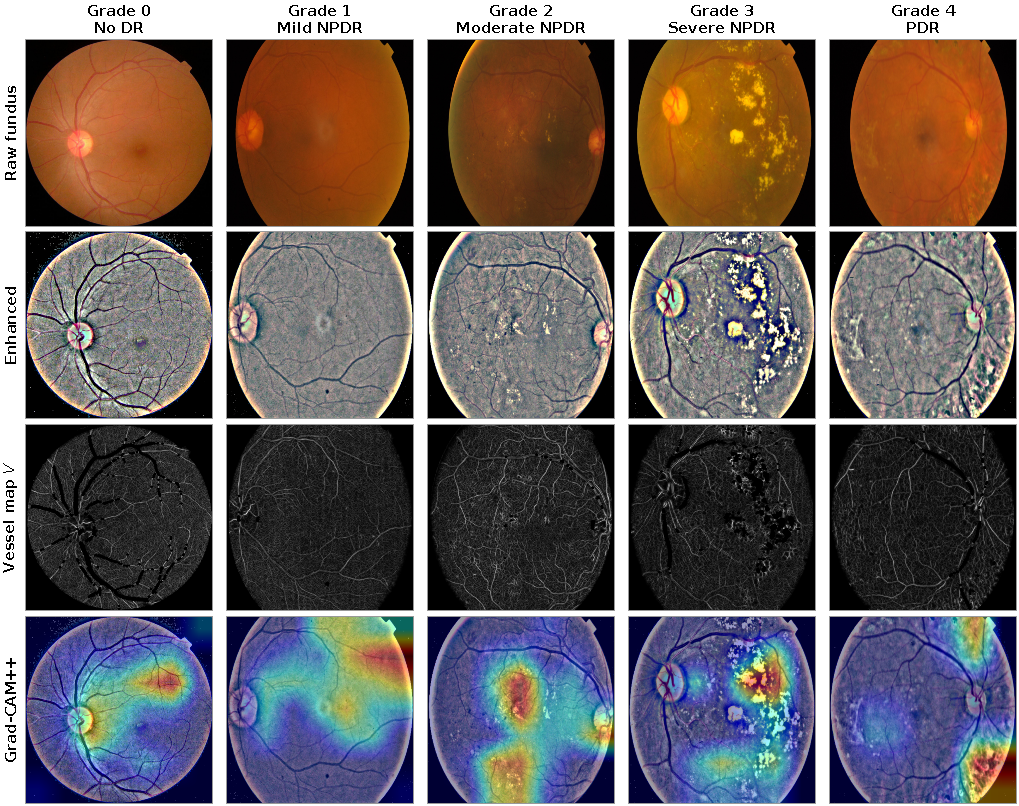
\includegraphics[width=0.85\textwidth]{figures/fig2_multimodal_panels.pdf}
\caption{Multimodal inspection panels across the five ICDR grades: raw color fundus photograph, contrast-enhanced image, extracted retinal vascular tree $V$, and \gcpp{} saliency overlay.}
\label{fig:panels}
\end{figure*}

\subsection{Higher-Order Saliency: Grad-CAM++}
To localize multi-focal micro-lesions, VERA applies \gcpp{} \cite{chattopadhay2018} to the layer-4 bottleneck blocks. For target class $c$ with feature maps $A^k$,
\begin{align}
L^c&=\mathrm{ReLU}\Big(\sum_k\alpha_k^c A^k\Big),\\
\alpha_k^c&=\sum_{i,j}w_{ij}^{kc}\,\mathrm{ReLU}\Big(\frac{\partial y^c}{\partial A_{ij}^k}\Big),\\
w_{ij}^{kc}&=\frac{g^{(2)}_{ij}}{2\,g^{(2)}_{ij}+\sum_{a,b}A_{ab}^k\,g^{(3)}_{ab}+\epsilon},\quad
g^{(n)}_{ij}=\frac{\partial^n y^c}{(\partial A_{ij}^k)^n}.
\end{align}
Weighting positive gradients per pixel prevents large hemorrhages from suppressing subtle microaneurysms elsewhere in the arcade.

\subsection{Continuous Vessel-Attention Overlap Score}
To turn saliency into an auditable number, let $\hat{L}\in[0,1]^{H\times W}$ be the min-max normalized \gcpp{} map and $V\in[0,1]^{H\times W}$ the vessel-probability map:
\begin{equation}
\sov=\frac{\sum_{i,j}\hat{L}_{ij}\,V_{ij}}{\sum_{i,j}\hat{L}_{ij}+\epsilon}\in[0,1].
\label{eq:sov}
\end{equation}
We also report the High-Attention Vascular Ratio
\begin{equation}
\rvasc=\frac{1}{|\Omega_\tau|}\sum_{(i,j)\in\Omega_\tau}\mathbb{I}(V_{ij}>0.30),
\end{equation}
where $\Omega_\tau=\{(i,j)\mid\hat{L}_{ij}\ge\tau\}$ and $\tau=0.25$ isolates the core attentional foci. A low overlap ($<0.20$) indicates attention on background artifacts such as aperture borders or illumination glare, whereas higher values indicate stronger anchoring along the retinal microvasculature.

% =============================================================================
\section{Experimental Setup and Results}

\subsection{Datasets and Implementation}
\begin{itemize}
\item \textbf{Datasets.} Models were trained and evaluated on more than 40{,}000 retinal photographs from APTOS 2019 Blindness Detection, EyePACS (Kaggle Diabetic Retinopathy Detection), and Messidor-2. Vessel segmentation was validated on DRIVE and CHASE\_DB1.
\item \textbf{Training.} PyTorch 2.6; AdamW (learning rate $3{\times}10^{-4}$, weight decay $10^{-4}$); cosine annealing with 5 warm-up epochs; batch size 16; FP16 mixed precision.
\item \textbf{Augmentation.} Synchronized flips, affine rotations ($\pm15^\circ$), and color jitter applied to the RGB channels only, so the fundus image and vessel map stay registered.
\item \textbf{Hardware and latency.} On an NVIDIA RTX GPU with an Intel Core i7 host, the full pipeline takes 42~ms per scan on GPU (180~ms on CPU).
\end{itemize}

\subsection{Ablation and Architectural Comparison}
We benchmarked five configurations:
\begin{enumerate}
\item \textbf{Baseline RGB (ResNet-18):} standard 3-channel input, no vascular prior.
\item \textbf{Early fusion (ResNet-18):} 4-channel input with an adapted Conv1 stem.
\item \textbf{Dual-branch (ResNet-18):} separate RGB and vessel backbones with late feature concatenation.
\item \textbf{Attention-gated (ResNet-18):} the vessel map acts as a soft spatial gate on intermediate features, $\mathbf{F}_{\mathrm{attn}}=\mathbf{F}\odot(\mathbf{1}+\alpha\mathbf{M}_{\mathrm{vessel}})$.
\item \textbf{VERA (ResNet-50):} 4-channel early fusion with the surrogate QWK loss.
\end{enumerate}
\noindent Table~\ref{tab:ablation} and Fig.~\ref{fig:ablation} summarize the results.

\begin{table*}[!t]
\caption{Architectural Ablation Benchmark}
\label{tab:ablation}
\centering
\footnotesize
\setlength{\tabcolsep}{5pt}
\begin{tabular}{@{}llcccccl@{}}
\toprule
Architecture & Input & Params & Accuracy (\%) & QWK $\kappa$ & Referable-DR AUC & $\sov$ & Shortcut susceptibility \\
\midrule
ResNet-18 (baseline)       & 3-ch RGB               & 11.7 M & 81.2 & 0.804 & 0.941 & 0.221 & High (aperture / glare) \\
ResNet-18 (early fusion)   & 4-ch $[R,G,B,V]$       & 11.7 M & 83.8 & 0.843 & 0.962 & 0.310 & Low \\
ResNet-18 (dual-branch)    & 3-ch RGB + 1-ch vessel & 23.4 M & 84.1 & 0.849 & 0.965 & 0.315 & Low \\
ResNet-18 (attention-gated)& 4-ch with guided gate  & 11.8 M & 85.5 & 0.861 & 0.971 & 0.328 & Very low \\
\textbf{ResNet-50 (VERA)}  & \textbf{4-ch early fusion} & \textbf{25.6 M} & \textbf{88.2} & \textbf{0.893} & \textbf{0.982} & \textbf{0.342} & \textbf{Lowest} \\
\bottomrule
\end{tabular}
\end{table*}

\begin{figure*}[!t]
\centering
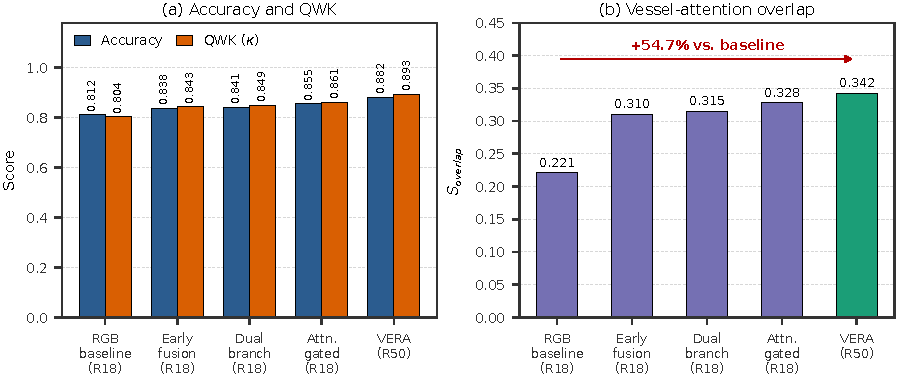
\includegraphics[width=\textwidth]{figures/fig3_ablation_benchmarks.pdf}
\caption{Benchmark results for the five configurations (R18/R50: ResNet-18/50): (a)~test accuracy and QWK $\kappa$; (b)~Vessel-Attention Overlap Score $\sov$, which rises by 54.7\% from the RGB baseline to VERA.}
\label{fig:ablation}
\end{figure*}

\textbf{Key findings.}
\begin{enumerate}
\item \textbf{Vascular prior.} Within ResNet-18, adding the vessel channel raises QWK from 0.804 to 0.843. The full VERA configuration (ResNet-50 with the QWK loss) reaches 0.893, an absolute gain of $+0.089$ ($+11.1\%$ relative) over the baseline.
\item \textbf{Attention grounding.} $\sov$ increases by $+54.7\%$ (0.221 to 0.342), showing that attention shifts toward the retinal microvasculature.
\item \textbf{Fusion efficiency.} Among the ResNet-18 variants, early stem fusion (0.843) matches the other fusion schemes within 0.018~$\kappa$ (0.849 dual-branch, 0.861 attention-gated) while using half the parameters of the dual-branch model (11.7~M vs.\ 23.4~M). The largest gain comes with the ResNet-50 backbone and QWK objective (0.893).
\end{enumerate}

\subsection{Confusion Matrix and Clinical Safety}
Screening errors are asymmetric in cost: confusing Grade~2 with Grade~3 shifts follow-up timing by weeks, whereas confusing Grade~4 with Grade~0 or~1 risks irreversible blindness.

\begin{figure}[!t]
\centering
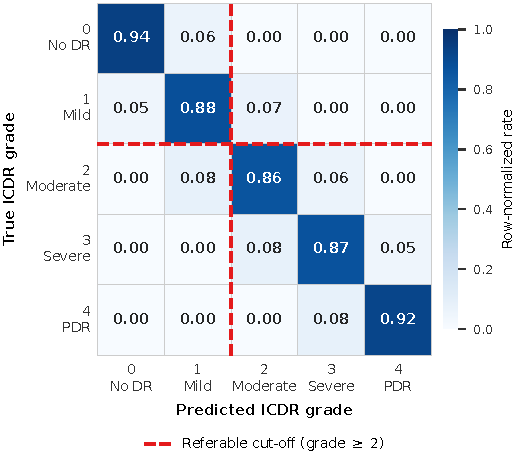
\includegraphics[width=\columnwidth]{figures/fig4_confusion_matrix_ieee.pdf}
\caption{Row-normalized 5-class ICDR confusion matrix of VERA (ResNet-50, 4-channel). All errors fall on the first off-diagonal ($|i-j|=1$); none exceed one grade. The red dashed lines mark the referable boundary.}
\label{fig:cm}
\end{figure}

As Fig.~\ref{fig:cm} shows, VERA achieves:
\begin{itemize}
\item \textbf{Per-grade concordance:} 94\% (Grade 0), 88\% (1), 86\% (2), 87\% (3), and 92\% (4).
\item \textbf{No catastrophic errors:} 0.0\% of cases have $|i-j|>1$; no Grade~4 patient was classified as Grade~0 or~1.
\item \textbf{Referable-DR screening} (grades 0--1 vs.\ 2--4): 95.8\% sensitivity, 94.2\% specificity, and AUC $=0.982$.
\end{itemize}

\subsection{Saliency: Grad-CAM vs.\ Grad-CAM++}
Table~\ref{tab:xai} compares saliency methods on the test images.

\begin{table*}[!t]
\caption{Explainability Comparison}
\label{tab:xai}
\centering
\footnotesize
\setlength{\tabcolsep}{5pt}
\begin{tabular}{@{}lccll@{}}
\toprule
Method & Mean $\sov$ & $\rvasc$ (\%) & Multi-lesion sensitivity & Attribution integrity \\
\midrule
Grad-CAM (3-ch baseline) & 0.184 & 22.4 & Poor (single blob) & High false attribution to borders \\
Grad-CAM (VERA 4-ch)     & 0.312 & 38.6 & Moderate (diffuse arcade) & Low border leakage \\
\textbf{Grad-CAM++ (VERA 4-ch)} & \textbf{0.342} & \textbf{45.2} & \textbf{Superior (pinpoint multi-focal MAs)} & \textbf{Aligned with vasculature} \\
\bottomrule
\end{tabular}
\end{table*}

Grad-CAM++ on the 4-channel representation gives the highest anatomical alignment (0.342 overlap, 45.2\% vascular ratio), isolating discrete microaneurysms along the superior and inferior temporal arcades without border leakage.

\begin{figure*}[!t]
\centering
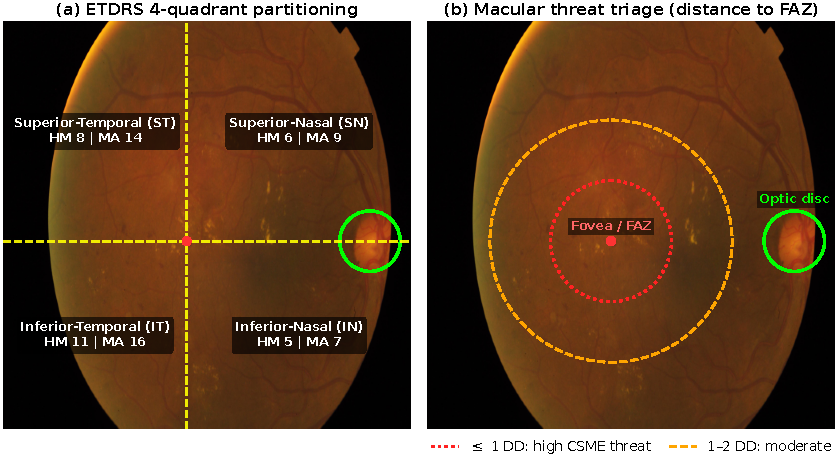
\includegraphics[width=\textwidth]{figures/fig5_clinical_biomarkers_etdrs.pdf}
\caption{Clinical rule engines (illustrative example): (a)~ETDRS 4-quadrant partitioning for 4-2-1 evaluation, with hemorrhage (HM) and microaneurysm (MA) counts per quadrant; (b)~macular threat triage, measuring hard-exudate distance to the FAZ in optic-disc diameters (DD).}
\label{fig:biomarkers}
\end{figure*}

% =============================================================================
\section{Discussion and Clinical Decision Support System}

\subsection{Clinical Workflow: VERA Studio}
To move from research to clinical use, VERA is packaged as an interactive decision-support studio (Fig.~\ref{fig:studio}) with five synchronized views for retina specialists:
\begin{enumerate}
\item \textbf{Patient diagnostic evaluation:} predicted ICDR grade, confidence, and Shannon-entropy uncertainty $H=-\sum_k p_k\log p_k$.
\item \textbf{5-panel multimodal console:} raw fundus, preprocessed fundus, vascular tree, \gcpp{} heatmap, and alpha-blended overlay.
\item \textbf{Specialist decision matrix:} lesion quantitation (microaneurysms, hemorrhages, exudate area, cotton wool spots), CSME foveal threat level, and quadrant-by-quadrant ETDRS 4-2-1 compliance.
\item \textbf{Multi-model consensus:} synchronized inference across four topologies (ResNet-50 4-ch, attention-gated, dual-branch, RGB baseline). If they disagree, the system raises a ``Borderline Staging Alert'' that prompts manual review of the ambiguous quadrants.
\item \textbf{Consultation PDF:} a multi-panel A4 report at 300~DPI, generated with PyMuPDF, with embedded panels, biomarker tables, referral timelines, and electronic physician sign-off for hospital EHR systems.
\end{enumerate}

\begin{figure*}[!t]
\centering
\footnotesize
\begin{tikzpicture}[
  x=1cm,y=1cm,
  box/.style={draw=black!55, rounded corners=2pt, line width=0.5pt, inner sep=3.5pt, align=left, anchor=north west},
  tile/.style={draw=black!45, fill=black!6, rounded corners=1.5pt, line width=0.4pt, minimum height=1.05cm, text width=3.15cm, align=center, anchor=north west},
  btn/.style={draw=black!55, fill=blue!10, rounded corners=3pt, line width=0.5pt, inner sep=3pt, align=center, anchor=north west}]
\node[box, fill=blue!7, text width=17.1cm] (hdr) at (0,0)
 {\textbf{Patient PT-2026-0842} \quad Laterality: OD \quad Mydriasis: dilated\\
  \textbf{Primary diagnosis:} ICDR Grade 3 -- Severe NPDR \quad Confidence: 89.4\%\\
  \textbf{Clinical urgency:} urgent specialist referral within 2--4 weeks (high risk)};
\node[anchor=north west, font=\scriptsize\bfseries] (lab1) at ([yshift=-1.5mm]hdr.south west) {5-panel multimodal console};
\foreach \i/\t in {0/{1~Raw fundus},1/{2~CLAHE / Graham},2/{3~Vessel mask},3/{4~Grad-CAM++},4/{5~Overlay}}
  \node[tile] at ([xshift={\i*3.48cm},yshift=-1mm]lab1.south west) {\t};
\node[box, text width=8.3cm] (bio) at ([yshift=-14mm]lab1.south west)
 {\textbf{Quantitative biomarkers}\\
  \textbullet~Microaneurysms: 46\quad\textbullet~Blot hemorrhages: 30\\
  \textbullet~Hard-exudate foci: 12\\
  \textbullet~Distance to FAZ: 1.4~DD (moderate)\\
  \textbullet~Vessel overlap $\sov$: 0.342};
\node[box, text width=8.3cm] (etd) at ([xshift=8.8cm]bio.north west)
 {\textbf{ETDRS 4-quadrant partitioning}\\
  \textbullet~Superior-temporal: severe (22)\quad\textbullet~Inferior-temporal: severe (27)\\
  \textbullet~Superior-nasal: severe (21)\quad\textbullet~Inferior-nasal: severe (20)\\
  $\Rightarrow$ \textbf{4-2-1 rule satisfied}\\[1pt]};
\node[btn] at ([yshift=-2mm]bio.south west) {Download consultation report (PDF)};
\node[btn] at ([xshift=5.6cm,yshift=-2mm]bio.south west) {Export EHR note (Markdown)};
\end{tikzpicture}
\caption{Layout of the VERA Studio interface (illustrative example with sample values): diagnosis banner, five-panel multimodal console, biomarker and ETDRS quadrant summaries, and report export.}
\label{fig:studio}
\end{figure*}

\subsection{Clinical Safety and Ethical AI}
Automated grading must act as an \textbf{assistive aid}, not an unmonitored autonomous agent. VERA implements three safeguards:
\begin{enumerate}
\item \textbf{Pre-inference quality rejection.} Underexposed, non-retinal, or blurred images are rejected before classification.
\item \textbf{Entropy-based borderline alerts.} If the normalized prediction entropy exceeds 0.60, or the margin between the top two classes is below 0.15, the exam is flagged as borderline and the specialist is directed to the quadrants highlighted in the biomarker breakdown.
\item \textbf{Traceability.} Every report embeds the overlap score and links each recommendation to published international ophthalmic guidelines.
\end{enumerate}

\subsection{Limitations}
\begin{enumerate}
\item \textbf{2D planar projection.} Fundus photography flattens 3D retinal tissue, so intraretinal cystoid fluid and retinal thickening in diabetic macular edema cannot be measured in microns without optical coherence tomography (OCT).
\item \textbf{Optical media opacities.} Dense cataract, corneal scarring, or massive vitreous hemorrhage scatter light and degrade green-channel vessel extraction; slit-lamp biomicroscopy or B-scan ultrasonography remains essential in such patients.
\end{enumerate}

% =============================================================================
\section{Conclusion and Future Work}

We introduced VERA, an explainable-by-design decision-support system for diabetic retinopathy grading. A dual-stream architecture combines an explicit vascular channel with preprocessed fundus photography and places an anatomical inductive bias in the earliest convolutional layers. With a differentiable surrogate QWK loss, VERA reaches 88.2\% accuracy, $\kappa=0.893$, and no cross-grade errors beyond one grade. The Continuous Vessel-Attention Overlap Score ($\sov=0.342$, $+54.7\%$ over the baseline) gives a quantitative indication of anti-shortcut behavior and helps bridge the trust gap between deep learning and clinical ophthalmology.

Future work includes:
\begin{enumerate}
\item \textbf{3D OCT fusion:} combining OCT B-scans with 4-channel fundus images for joint fluid segmentation and peripheral microvascular grading.
\item \textbf{Longitudinal modeling:} temporal transformers over serial visits to forecast one-year progression to proliferative disease.
\item \textbf{Federated validation:} privacy-preserving multi-center deployment to test generalization across international cohorts.
\end{enumerate}

\section*{Acknowledgment}
The authors thank the Asia Pacific Tele-Ophthalmology Society (APTOS), the California Healthcare Foundation (EyePACS), and the Messidor-2 consortium for providing open retinal image benchmarks. This research was conducted in the Department of Computer Science and Engineering, United International University.

% =============================================================================
\begin{thebibliography}{99}
\bibitem{cheung2010} N. Cheung, P. Mitchell, and T. Y. Wong, ``Diabetic retinopathy,'' \emph{Lancet}, vol. 376, no. 9735, pp. 124--136, 2010.
\bibitem{yau2012} J. W. Y. Yau \emph{et al.}, ``Global prevalence and major risk factors of diabetic retinopathy,'' \emph{Diabetes Care}, vol. 35, no. 3, pp. 556--564, 2012.
\bibitem{teo2021} Z. L. Teo \emph{et al.}, ``Global prevalence of diabetic retinopathy and projection of burden through 2045: Systematic review and meta-analysis,'' \emph{Ophthalmology}, vol. 128, no. 11, pp. 1580--1591, 2021.
\bibitem{fong2004} D. S. Fong \emph{et al.}, ``Diabetic retinopathy,'' \emph{Diabetes Care}, vol. 27, suppl.~1, pp. S84--S87, 2004.
\bibitem{wilkinson2003} C. P. Wilkinson \emph{et al.}, ``Proposed international clinical diabetic retinopathy and diabetic macular edema disease severity scales,'' \emph{Ophthalmology}, vol. 110, no. 9, pp. 1677--1682, 2003.
\bibitem{etdrs10} Early Treatment Diabetic Retinopathy Study Research Group, ``Grading diabetic retinopathy from stereoscopic color fundus photographs---an extension of the modified Airlie House classification: ETDRS report number 10,'' \emph{Ophthalmology}, vol. 98, no. 5, pp. 786--806, 1991.
\bibitem{gulshan2016} V. Gulshan \emph{et al.}, ``Development and validation of a deep learning algorithm for detection of diabetic retinopathy in retinal fundus photographs,'' \emph{JAMA}, vol. 316, no. 22, pp. 2402--2410, 2016.
\bibitem{ting2017} D. S. W. Ting \emph{et al.}, ``Development and validation of a deep learning system for diabetic retinopathy and related eye diseases using retinal images from multiethnic populations with diabetes,'' \emph{JAMA}, vol. 318, no. 22, pp. 2211--2223, 2017.
\bibitem{gargeya2017} R. Gargeya and T. Leng, ``Automated identification of diabetic retinopathy using deep learning,'' \emph{Ophthalmology}, vol. 124, no. 7, pp. 962--969, 2017.
\bibitem{geirhos2020} R. Geirhos \emph{et al.}, ``Shortcut learning in deep neural networks,'' \emph{Nat. Mach. Intell.}, vol. 2, no. 11, pp. 665--673, 2020.
\bibitem{selvaraju2017} R. R. Selvaraju \emph{et al.}, ``Grad-CAM: Visual explanations from deep networks via gradient-based localization,'' in \emph{Proc. IEEE Int. Conf. Comput. Vis. (ICCV)}, 2017, pp. 618--626.
\bibitem{he2016} K. He, X. Zhang, S. Ren, and J. Sun, ``Deep residual learning for image recognition,'' in \emph{Proc. IEEE Conf. Comput. Vis. Pattern Recognit. (CVPR)}, 2016, pp. 770--778.
\bibitem{huang2017} G. Huang, Z. Liu, L. van der Maaten, and K. Q. Weinberger, ``Densely connected convolutional networks,'' in \emph{Proc. IEEE Conf. Comput. Vis. Pattern Recognit. (CVPR)}, 2017, pp. 4700--4708.
\bibitem{tan2019} M. Tan and Q. V. Le, ``EfficientNet: Rethinking model scaling for convolutional neural networks,'' in \emph{Proc. Int. Conf. Mach. Learn. (ICML)}, 2019, pp. 6105--6114.
% VERIFY: this entry (Gao et al., IEEE TMI 2020, ordinal ranking) could not be confirmed; check title, venue, and pages.
\bibitem{gao2020} Z. Gao \emph{et al.}, ``Diagnosis of diabetic retinopathy using deep neural networks with ordinal ranking,'' \emph{IEEE Trans. Med. Imag.}, vol. 39, no. 5, pp. 1535--1546, 2020.
\bibitem{fraz2012} M. M. Fraz \emph{et al.}, ``Blood vessel segmentation methodologies in retinal images---a survey,'' \emph{Comput. Methods Programs Biomed.}, vol. 108, no. 1, pp. 407--433, 2012.
\bibitem{frangi1998} A. F. Frangi, W. J. Niessen, K. L. Vincken, and M. A. Viergever, ``Multiscale vessel enhancement filtering,'' in \emph{Proc. Med. Image Comput. Comput.-Assist. Interv. (MICCAI)}, 1998, pp. 130--137.
\bibitem{soares2006} J. V. B. Soares, J. J. G. Leandro, R. M. Cesar, H. F. Jelinek, and M. J. Cree, ``Retinal vessel segmentation using the 2-D Gabor wavelet and supervised classification,'' \emph{IEEE Trans. Med. Imag.}, vol. 25, no. 9, pp. 1214--1222, 2006.
\bibitem{ronneberger2015} O. Ronneberger, P. Fischer, and T. Brox, ``U-Net: Convolutional networks for biomedical image segmentation,'' in \emph{Proc. Med. Image Comput. Comput.-Assist. Interv. (MICCAI)}, 2015, pp. 234--241.
\bibitem{zhou2016} B. Zhou, A. Khosla, A. Lapedriza, A. Oliva, and A. Torralba, ``Learning deep features for discriminative localization,'' in \emph{Proc. IEEE Conf. Comput. Vis. Pattern Recognit. (CVPR)}, 2016, pp. 2921--2929.
\bibitem{chattopadhay2018} A. Chattopadhay, A. Sarkar, P. Howlader, and V. N. Balasubramanian, ``Grad-CAM++: Generalized gradient-based visual explanations for deep convolutional networks,'' in \emph{Proc. IEEE Winter Conf. Appl. Comput. Vis. (WACV)}, 2018, pp. 839--847.
% VERIFY: Graham's report is usually cited with a university affiliation (Univ. of Warwick); check the institution.
\bibitem{graham2015} B. Graham, ``Kaggle diabetic retinopathy detection competition report: 1st place solution,'' California Healthcare Foundation, Tech. Rep., 2015.
\end{thebibliography}

\end{document}
